\chapter{Κατανάλωση Ισχύος Ψηφιακών Κυκλωμάτων}
\label{chap3}

\section{Εισαγωγή}
\label{chap3_Intro}

Η επιτακτική ανάγκη συρρίκνωσης των τρανζίστορ σε συνδυασμό με την ταυτόχρονη μείωση της τάσης λειτουργίας τους έχει αναδείξει ένα πολύ σημαντικό ζήτημα στα σύγχρονα ολοκληρωμένα κυκλώματα, αυτό της εμφάνισης βλαβών. Η βλάβη ενός στοιχείου του κυκλώματος μπορεί να έχει ως αποτέλεσμα την καθυστέρηση των υπολογισμών, καθιστώντας το σύστημα μη αποδοτικό, και στη χειρότερη περίπτωση την αλλοίωση των δεδομένων, καθιστώντας το μη αξιόπιστο. Για την αντιμετώπιση αυτών των βλαβών έχουν προταθεί και υλοποιηθεί πληθώρα μεθόδων, με σκοπό τον κατά το δυνατό μεγαλύτερο περιορισμό των επιπτώσεών τους. Στο παρόν κεφάλαιο γίνεται η θεωρητική προσέγγιση της κατανάλωσης ενέργειας των ψηφιακών κυκλωμάτων καθώς και η περιγραφή της σχέσης μεταξύ της εφαρμοζόμενης τάσης λειτουργίας και της πιθανότητας εμφάνισης βλαβών σε αυτά.

%----------------------------------------------------------%

\section{Κατανάλωση Ολοκληρωμένων Κυκλωμάτων}
\label{chap3_LowPowerSOC}

Αποτελεί γεγονός πως η πρόοδος της σχεδίασης των ψηφιακών κυκλωμάτων βαδίζει με γοργούς ρυθμούς. Όπως προέβλεπε ο νόμος του \en{Moore} \cite{moore2006progress} το 1975, το πλήθος των τρανζίστορ ενός ολοκληρωμένου (βαθμός ολοκλήρωσης) θα διπλασιάζεται κάθε δύο χρόνια. Παρότι τα τελευταία χρόνια θεωρήθηκε αρκετές φορές πως ο ρυθμός ολοκλήρωσης πρόκειται σύντομα να επιβραδυνθεί, η σχεδίαση ολοένα και μικρότερου μεγέθους τρανζίστορ συνεχίζει να επιβεβαιώνει το νόμο, καθιστώντας αυτό το στόχο ως κίνητρο έρευνας για τους κατασκευαστές μικροεπεξεργαστών \cite{moore2003no}. Από τα 130\nm – 45\nm μεγέθους τρανζίστορ που παρουσιάστηκαν την δεκαετία του 2000 η τεχνολογία των 14\nm αποτελεί πλέον γεγονός, ενώ οι κατασκευαστές έχουν ήδη ανακοινώσει πως σύντομα θα πραγματοποιηθεί η υλοποίηση τρανζίστορ μεγέθους 10\nm \cite{courtland2017moore}.
\par
Η ιλιγγιώδης αύξηση του πλήθους τρανζίστορ που εμπεριέχονται σε έναν επεξεργαστή (2-4 δισεκατομμύρια τρανζίστορ) είχε ώς συνέπεια τη μεγάλη αύξηση της καταναλισκόμενης ενέργειας και της εκλυόμενης θερμότητας, με τις συνέπειες που αυτή έχει στην ορθή λειτουργία των στοιχείων του. Στο γράφημα του Σχήματος \ref{fig:chap3_energy_per_tech} παρουσιάζεται τμήμα του άρθρου του \en{Dreslinski} και άλλων \cite{dreslinski2010near}, σχετικά με την εξέλιξη των ολοκληρωμένων κυκλωμάτων τα τελευταία χρόνια. Στο συγκεκριμένο γράφημα η καμπύλη μαύρου χρώματος αντιστοιχεί στη συνολική κατανάλωση ενέργειας του κυκλώματος (άξονας αριστερά). Τα δεδομένα παρουσιάζονται κανονικοποιημένα ως προς την περίπτωση κυκλώματος τεχνολογίας 250\nm. Στα πρώτα στάδια η μείωση του μεγέθους αποτέλεσε πολύ σημαντικό παράγοντα στην προσπάθεια περιορισμού της απώλειας ενέργειας. Όπως φαίνεται και από το γράφημα, η μετάβαση από τα 250\nm στο 180\nm προκάλεσε μείωση της καταναλισκόμενης ενέργειας πάνω από 50\%. Παρόλα αυτά, ο ρυθμός μείωσης της κατανάλωσης παρουσιάζει πτωτική τάση καθώς το μέγεθος των τρανζίστορ τείνει σε μερικές δεκάδες νανόμετρα.

\begin{figure}[!t]
    \centering
    \begin{subfigure}[t]{0.49\textwidth}
        \centering
        \fbox{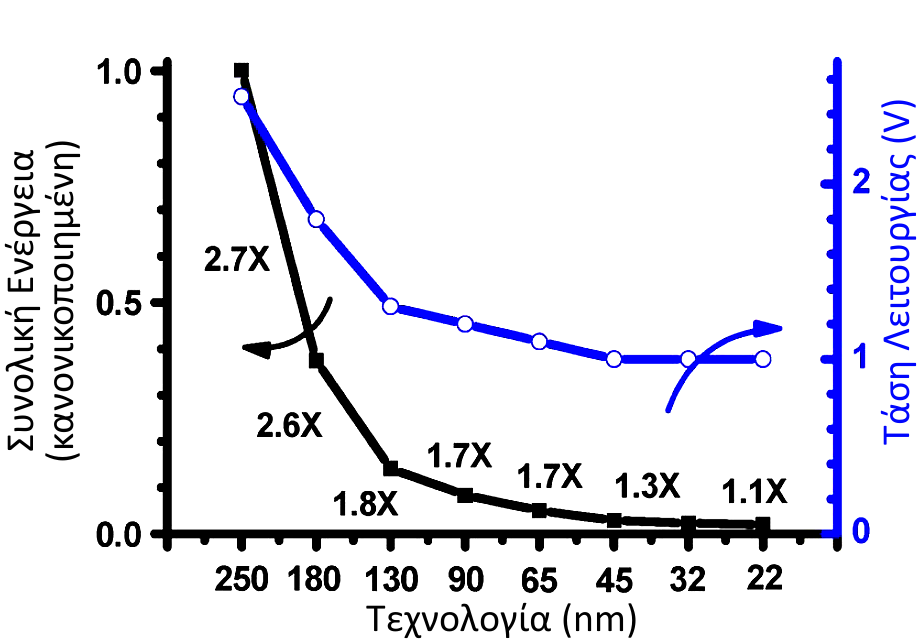
\includegraphics[width=0.98\linewidth, clip=true]{\researchesDIR/chap3_tech_energy.png}}
        \caption[Συνολική ενέργεια $\&$ τάση λειτουργίας]{Συνολική ενέργεια $\&$ τάση λειτουργίας \cite{dreslinski2010near}}
        \label{fig:chap3_energy_per_tech}
    \end{subfigure}%
    \hfill
    \begin{subfigure}[t]{0.49\textwidth}
        \centering
        \fbox{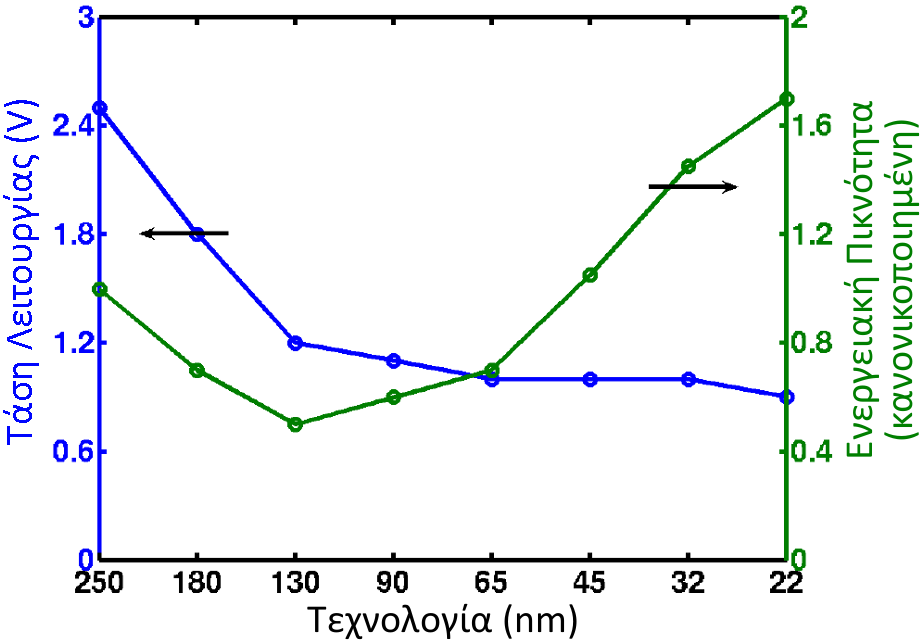
\includegraphics[width=0.98\linewidth, clip=true]{\researchesDIR/chap3_tech_vdd_ed.png}}
        \caption[Τάση λειτουργίας $\&$ πυκνότητα ενέργειας]{Τάση λειτουργίας $\&$ πυκνότητα ενέργειας \cite{pinckney2012assessing}}
        \label{fig:chap3_vdd_per_tech}
    \end{subfigure}
    \caption{Μεταβολή της τάσης λειτουργίας και της ενέργειας με τη συρρίκνωση της τεχνολογίας. Τα αποτελέσματα της συνολικής ενέργειας και της πυκνότητας ενέργειας εμφανίζονται κανονικοποιημένα ως προς τη περίπτωση των 250\nm.}
    \label{fig:chap3_Technology}
\end{figure}

Όπως αναφέρει και η μελέτη του \en{Pinckney} και άλλων \cite{pinckney2012assessing}, η αύξηση των ρευμάτων διαρροής των τρανζίστορ κατέστησε αδύνατη τη μείωση της τάσης κατωφλίου από το σημείο των 65\nm και έπειτα, επομένως και τη μείωση της τάσης λειτουργίας του κυκλώματος, όπως φανερώνει και η καμπύλη μπλε απόχρωσης στα Σχήματα \ref{fig:chap3_energy_per_tech} και \ref{fig:chap3_vdd_per_tech}. Η αδυναμία περαιτέρω μείωσης της τάσης λειτουργίας σε συνδυασμό με τη συνεχόμενη αύξηση της κλίμακας ολοκλήρωση έχει ως αποτέλεσμα την αύξηση της πυκνότητας ενέργειας, δηλαδή της ενέργειας που δαπανάται ανά τετραγωνικό χιλιοστό (καμπύλη πράσινης απόχρωσης Σχήματος \ref{fig:chap3_vdd_per_tech}). Αυτή η αύξηση συνεπάγεται την υπερθέρμανση ορισμένων κρίσιμων τμημάτων του ολοκληρωμένου, με κίνδυνο εμφάνισης βλαβών σε αυτά μελλοντικά. Η κατανάλωση ισχύος ενός κυκλώματος (κατανάλωση ενέργειας στο χρόνο) οφείλεται σε μία πληθώρα στοιχείων, και μπορεί να διαχωριστεί σε δύο βασικές κατηγορίες:
\par
\textit{\textbf{Δυναμική:}} Η ισχύς που καταναλώνεται όταν ένας κόμβος (τρανζίστορ) του κυκλώματος πραγματοποιεί μετάβαση κατάστασης από 0 σε 1 και αντίστροφα. Όταν στο κύκλωμα εφαρμόζεται η ονομαστική τάση λειτουργίας οι καταναλώσεις αυτού του είδους αποτελούν τον πιο σημαντικό παράγοντα στη συνολική κατανάλωση ισχύος του συστήματος.
\par
\textit{\textbf{Στατική:}} Η ισχύς που καταναλώνεται σε ένα κύκλωμα όταν δεν πραγματοποιείται μεταβολή της κατάστασής στους κόμβους (τρανζίστορ) του, και οφείλεται στα ρεύματα διαρροής των τρανζίστορ. Καθώς η τεχνολογία συρρικνώνεται και η τάση λειτουργίας μειώνεται οι καταναλώσεις αυτού του είδους αποτελούν πολύ σημαντικό παράγοντα στη συνολική κατανάλωση ισχύος, σχεδόν όσο και η δυναμική.\par
\par

\begin{figure}[!t]
    \centering
    \begin{subfigure}[t]{0.49\textwidth}
        \centering
        \fbox{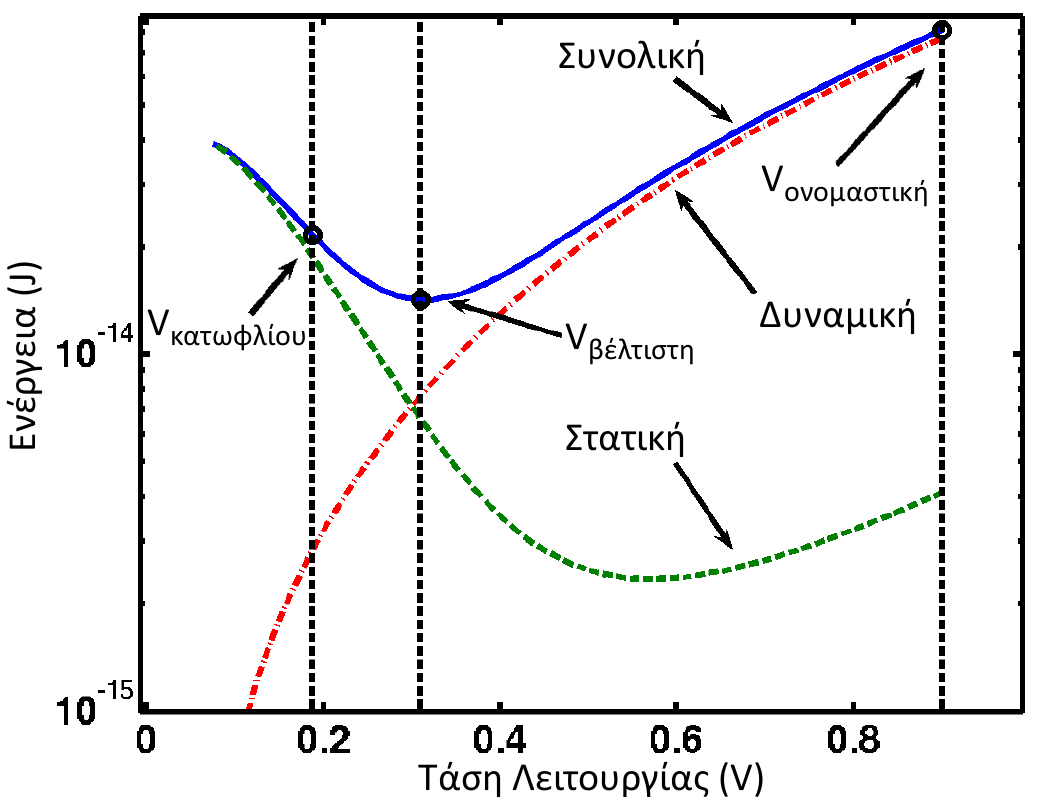
\includegraphics[width=0.98\linewidth, clip=true]{\researchesDIR/chap3_vdd_energy.png}}
        \caption{Συνολική, δυναμική $\&$ στατική κατανάλωση}
        \label{fig:chap3_energy_per_vdd}
    \end{subfigure}%
    \hfill
    \begin{subfigure}[t]{0.49\textwidth}
        \centering
        \fbox{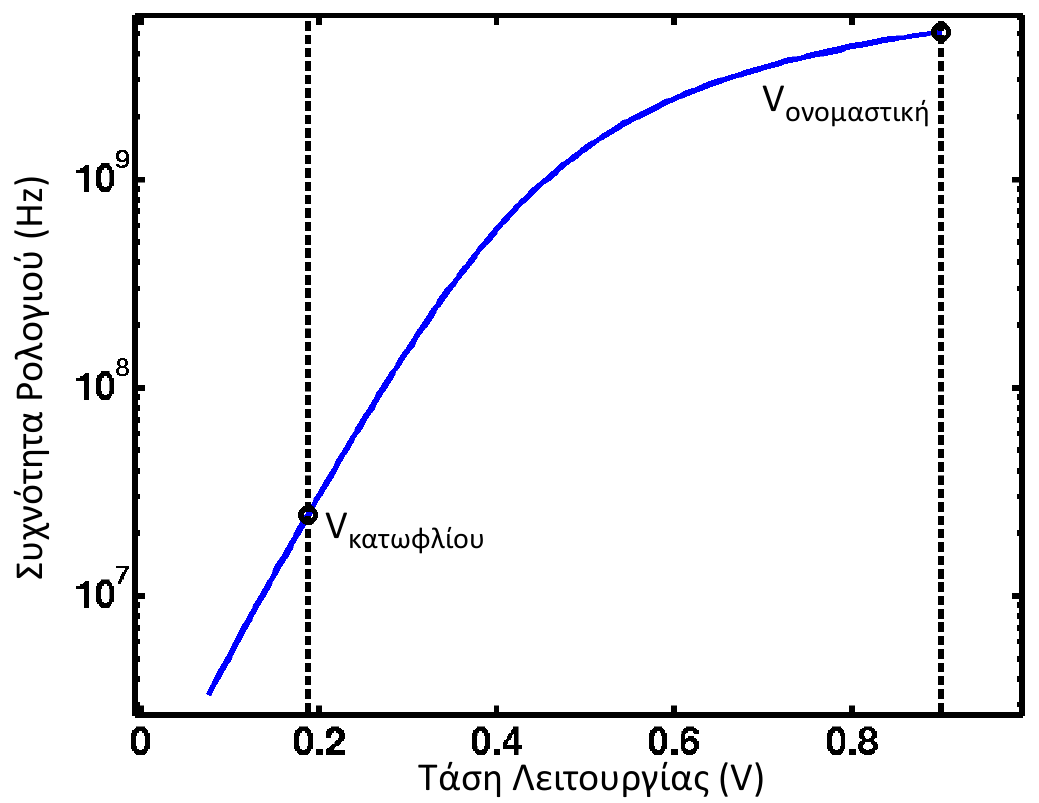
\includegraphics[width=0.98\linewidth, clip=true]{\researchesDIR/chap3_vdd_freq.png}}
        \caption{Μέγιστη συχνότητα λειτουργίας}
        \label{fig:chap3_freq_per_vdd}
    \end{subfigure}
    \caption[Μεταβολή της καταναλισκόμενης ενέργειας και της μέγιστης συχνότητας ρολογιού σε διαφορετικές τάσεις λειτουργίας ενός κυκλώματος τεχνολογίας 32\nm]{Μεταβολή της καταναλισκόμενης ενέργειας και της μέγιστης συχνότητας ρολογιού σε διαφορετικές τάσεις λειτουργίας ενός κυκλώματος τεχνολογίας 32\nm \cite{pinckney2012assessing}}
    \label{fig:chap3_Vdd}
\end{figure}

Στο γράφημα του Σχήματος \ref{fig:chap3_energy_per_vdd} παρουσιάζεται η σχέση μεταξύ δυναμική και στατικής κατανάλωσης για διαφορετικά επίπεδα τάσης λειτουργίας ενός ολοκληρωμένου τεχνολογίας 32\nm, όπως αναφέρεται στην ίδια μελέτη του \en{Pinckney} \cite{pinckney2012assessing}. Αντίστοιχα, το γράφημα του Σχήματος \ref{fig:chap3_freq_per_vdd} παρουσιάζει τη μεταβολή της συχνότητας σε αυτό το εύρος τάσης. Από το πρώτο γράφημα γίνεται ξεκάθαρο πως με τη μείωση της τάσης λειτουργίας έως το βέλτιστο σημείο η συνολική κατανάλωση ενέργειας μειώνεται (καμπύλη μπλε απόχρωσης). Χαρακτηριστικό είναι το γεγονός πως για τάση λειτουργίας μικρότερη του βέλτιστου παρουσιάζεται σημαντική αύξηση της στατικής κατανάλωσης (καμπύλη πράσινης απόχρωσης), σε αντίθεση με τη δυναμική (καμπύλη κόκκινης απόχρωσης) η οποία συνεχώς μειώνεται. Στο σημείο που η στατική κατανάλωση ισούται με τη δυναμική η τάση λειτουργίας αποτελεί τη βέλτιστη επιλογή για τη μείωση της συνολικής καταναλισκόμενης ενέργειας. Παράλληλα, με τη μείωση της τάσης λειτουργίας αναπόφευκτα επιβάλλεται και η πτώση της συχνότητας ρολογιού εξαιτίας της αύξησης του χρόνου εναλλαγής καταστάσεων των τρανζίστορ. Η μείωση αυτή παρουσιάζεται στο δεύτερο γράφημα (Σχήμα \ref{fig:chap3_freq_per_vdd}).

%----------------------------------------------------------%

\section{Δυναμική Μεταβολή Τάσης και Συχνότητας}
\label{chap3_PowerReduction}

Ο σχεδιασμός ενός συστήματος μειωμένης κατανάλωσης μπορεί τα επιτευχθεί μέσω του συνδυασμού κατάλληλων τεχνικών στα διαφορετικά επίπεδα που το αποτελούν. Ξεκινώντας από το χαμηλότερο επίπεδο, αυτό της σχεδίασης ψηφιακών κυκλωμάτων, έως και το ανώτερο επίπεδο, της σχεδίασης του λογισμικού που εκτελείται στο κύκλωμα, είναι αναγκαίο να επιτυγχάνεται η αύξηση της απόδοσης με ταυτόχρονη μείωση του κόστους που έχει σε ενέργεια. Από τις μελέτες που παρουσιάστηκαν αλλά και πολλές ακόμη που έχουν διενεργηθεί τα τελευταία χρόνια σε επίπεδο υλικού, προκύπτει πως για να επιτευχθεί η μείωση της καταναλισκόμενης ενέργειας ενός ολοκληρωμένου κυκλώματος απαιτείται η εφαρμογή κατάλληλου συνδυασμού τάσης και συχνότητας λειτουργίας \cite{zhai2009energy, lorente2014analyzing, de2016near}. Το γεγονός αυτό εκμεταλλεύονται οι σύγχρονοι υπερβαθμωτοί επεξεργαστές οι οποίοι σχεδιάζονται κατά τέτοιο τρόπο ώστε να μπορούν να λειτουργούν σε διαφορετικά επίπεδα τάσης και συχνότητας ανά χρονικά διαστήματα. Η τεχνική αυτή ονομάζεται Δυναμική Μεταβολή Τάσης και Συχνότητας (\en{DVFS}) και αποτελεί πλέον αναπόσπαστο κομμάτι τους.
\par
Η ιδέα του \en{DVFS} βασίζεται στο γεγονός ότι ο φόρτος εργασίας μεταβάλλεται κατά το χρόνο λειτουργίας ενός επεξεργαστή. Επομένως, στις χρονικές περιόδους όπου η απαιτούμενη επεξεργαστική ισχύς είναι μικρή μπορεί να γίνει υποβάθμιση της απόδοσης του συστήματος ώστε να μειωθεί η δυναμική κατανάλωση του, η οποία υπολογίζεται από τη σχέση:

\begin{equation}
    \label{eqn:chap3_dynamic_power}
    P = CV^{2}f
\end{equation}

\noindent
όπου $C$ είναι η συνολική χωρητικότητα του κυκλώματος, $V$ η τάση λειτουργίας, και $f$ η συχνότητα ρολογιού.
\par
Στη σχέση \eqref{eqn:chap3_dynamic_power} η χωρητικότητα αποτελεί σταθερό παράγοντα ενός κυκλώματος, εν αντιθέσει με τη τάση και τη συχνότητα τα οποία μπορούν να μεταβάλλονται. Συνεπώς, για να επιτευχθεί η μείωση της κατανάλωσης ισχύος πρέπει να γίνει κατάλληλη προσαρμογή των παραγόντων τάση και συχνότητα. Όπως είναι φανερό, μία μικρή μείωση της τάσης λειτουργίας μπορεί να οδηγήσει σε σημαντική μείωση της δυναμικής κατανάλωσης ισχύος. Στο γράφημα του Σχήματος \ref{fig:chap3_intel_ntv} παρουσιάζεται η μεταβολή της συχνότητας και της κατανάλωσης ισχύος ενός επεξεργαστή τεχνολογίας 32\nm, για διαφορετικά επίπεδα τάσης λειτουργίας, όπως παρουσιάζονται στο άρθρο των \en{De}, \en{Vangal} και \en{Krishnamurthy} \cite{de2016near}.

\begin{figure}[h]
    \centering
    \fbox{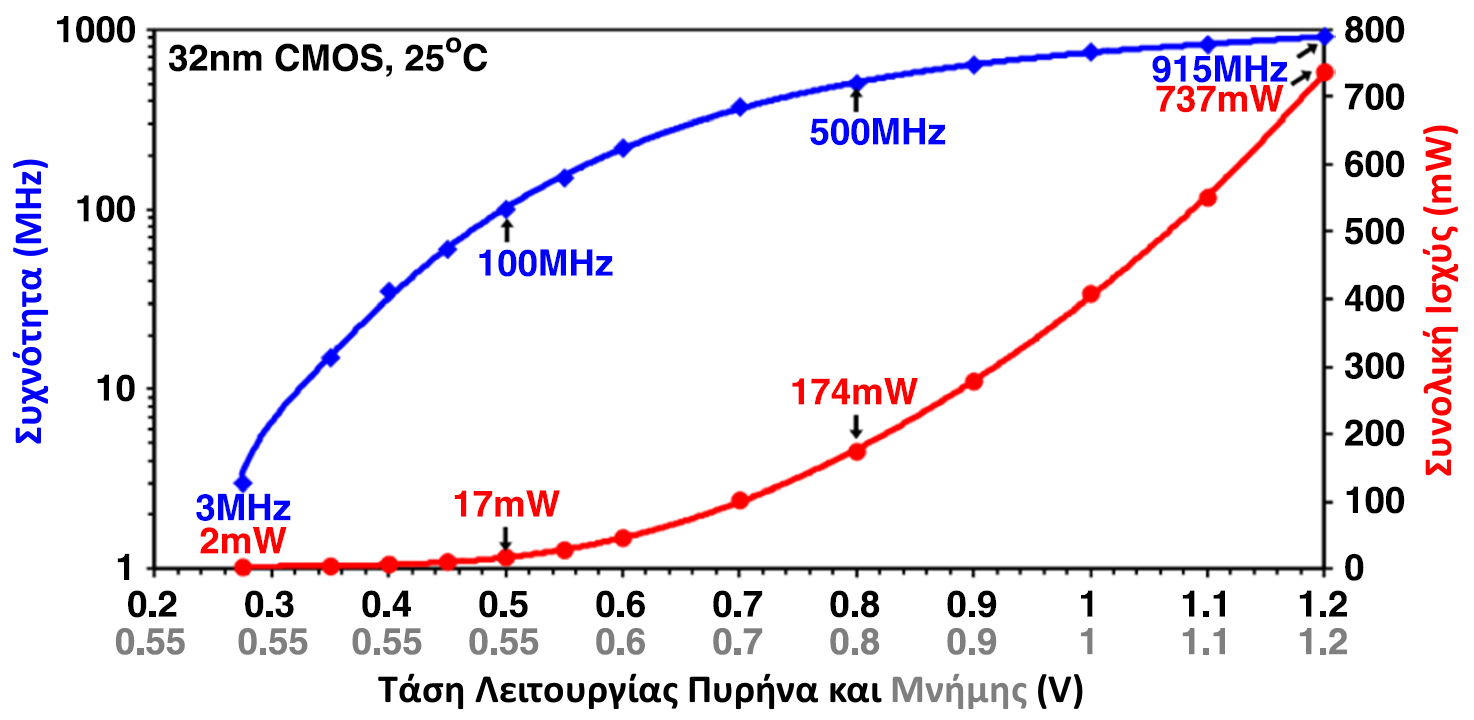
\includegraphics[width=0.85\linewidth, clip=true]{\researchesDIR/chap3_intel_ntv.png}}
    \caption[Σχέση συχνότητας και ισχύος με τις μεταβολές του επιπέδου τάσης λειτουργίας ενός επεξεργαστή τεχνολογίας 32\nm]{Σχέση συχνότητας και ισχύος με τις μεταβολές του επιπέδου τάσης λειτουργίας ενός επεξεργαστή τεχνολογίας 32\nm \cite{de2016near}}
    \label{fig:chap3_intel_ntv}
\end{figure}

%----------------------------------------------------------%

\section{Δυναμικό Χαμηλού Επιπέδου και Βλάβες}
\label{chap3_LowLevelVccFaults}

Όπως αναφέρθηκε ήδη, η συρρίκνωση του μεγέθους των τρανζίστορ σε συνδυασμό με την αύξηση της ολοκλήρωσης των επεξεργαστών οδηγεί στην εμφάνιση βλαβών. Ιδιαίτερα, καθώς η τάση λειτουργίας των τρανζίστορ μειώνεται σημαντικά σε σχέση με την ονομαστική, με σκοπό τη μείωση της κατανάλωσης κατά το μέγιστο δυνατόν, ορισμένα από αυτά αρχίζουν να μην λειτουργούν με τον αναμενόμενο τρόπο. Τα πιο συνηθισμένα «θύματα» αυτής της μεγάλης μείωσης της τάσης λειτουργίας είναι οι κυψελίδες \en{SRAM} που αποτελούν τα στοιχεία μνήμης του ολοκληρωμένου. Εξαιτίας της μεγάλης επιφάνειας που καταλαμβάνουν τα στοιχεία μνήμης, συνηθίζεται να υλοποιούνται με μικρότερα και συνεπώς πιο ευάλωτα τρανζίστορ \cite{nassif2010resilience, gottscho2014power}. Αυτό έχει σαν συνέπεια να παρουσιάζουν είτε αστάθεια στη συμπεριφορά τους είτε να μην ανταποκρίνονται καθόλου σε επιθυμητές μεταβολές της κατάστασής τους. Στο Σχήμα \ref{fig:chap3_22nm_pfail} παρουσιάζεται τμήμα της μελέτης της \en{Ferreron} και άλλων \cite{ferreron2014block}, και όπως φανερώνει το γράφημα, η πιθανότητα μίας κυψελίδας \en{SRAM} να εμφανίσει βλάβη αυξάνεται μη γραμμικά καθώς η τάση λειτουργίας μειώνεται.

\begin{figure}[h]
    \centering
    \fbox{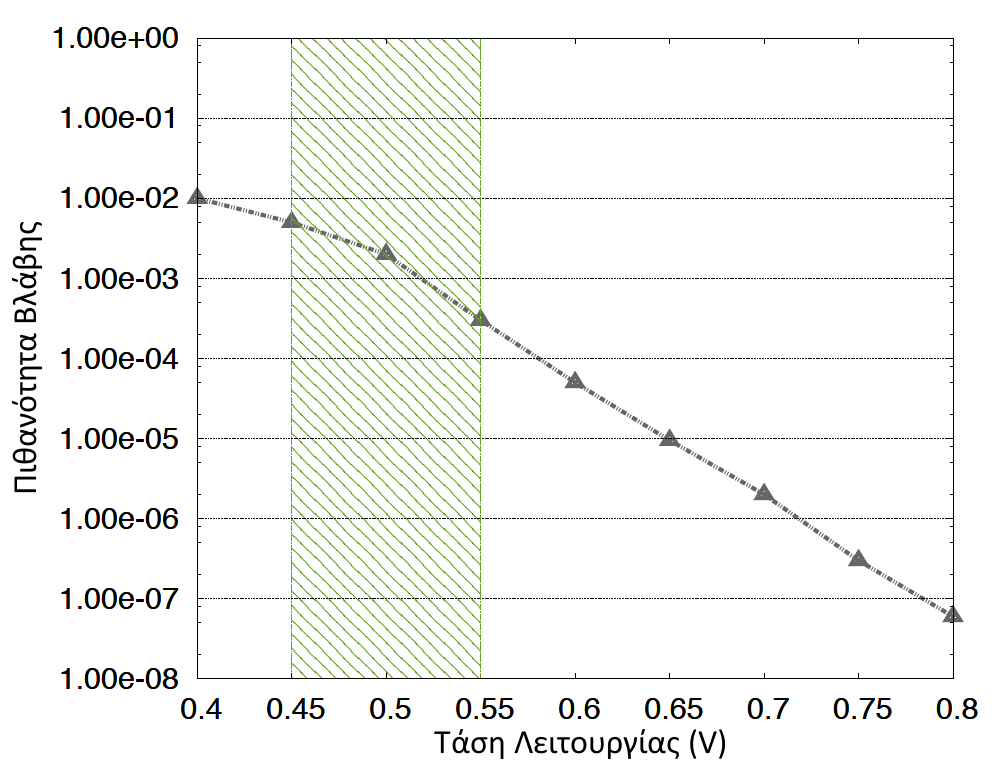
\includegraphics[width=0.7\linewidth, clip=true]{\researchesDIR/chap3_pfail_vdd_22nm.png}}
    \caption[Μεταβολή της πιθανότητα βλάβης μίας \en{SRAM} κυψελίδας στα 22\nm με τη μεταβολή της τάσης λειτουργίας]{Μεταβολή της πιθανότητα βλάβης μίας \en{SRAM} κυψελίδας στα 22\nm με τη μεταβολή της τάσης λειτουργίας \cite{ferreron2014block}}
    \label{fig:chap3_22nm_pfail}
\end{figure}

Με τη συρρίκνωση της τεχνολογίας η καμπύλη αυτή μετατοπίζεται προς τα επάνω, διότι τα τρανζίστορ γίνονται περισσότερο ευάλωτα. Όταν μία κυψελίδα περιέχει βλάβη χαρακτηρίζεται ως ελαττωματική, και τα δεδομένα που αποθηκεύονται σε αυτή αυτή είναι πιθανό να αλλοιωθούν. Επομένως, οι ελαττωματικές αυτές θέσεις ενός ολοκληρωμένου χαρακτηρίζονται ως σφάλματα \cite{nikolosTesting}.

%----------------------------------------------------------%

\section{Ανίχνευση/Διόρθωση Λαθών και Ανοχή Σφαλμάτων}
\label{chap3_FaultTaulerance}

Για την αντιμετώπιση των σφαλμάτων του συστήματος, τόσο κατά την κατασκευή όσο και κατά τη λειτουργία του, πραγματοποιείται κατάλληλος έλεγχος ώστε να εντοπίζονται εάν και σε ποια σημεία του κυκλώματος εμφανίζονται λάθη. Η διαδικασία αυτή αποκαλείται Ανίχνευση Σφαλμάτων και σε αρκετά συστήματα η εκτέλεσή της πραγματοποιείται σε διαφορετικά στιγμιότυπα της λειτουργίας τους.
\par
Η εμφάνιση σφαλμάτων μπορεί να οδηγήσει είτε σε απλή επιβάρυνση του χρόνου εκτέλεσης των προγραμμάτων (μείωση της απόδοσης), το οποίο θα έχει και ως συνέπεια την αύξηση της καταναλισκόμενης ενέργειας, είτε την παραγωγή λανθασμένων αποτελεσμάτων. Στην πρώτη περίπτωση, παρότι η σωστή εκτέλεση του προγράμματος δεν τίθεται σε κίνδυνο, χρησιμοποιούνται κατάλληλες τεχνικές ώστε να περιορίζεται η επιβάρυνση της απόδοσης κατά το μέγιστο δυνατόν. Αντιθέτως, στη δεύτερη περίπτωση η μη αντιμετώπιση των ελαττωματικών στοιχείων μνήμης θα οδηγούσε σε υλοποίηση ενός μη αξιόπιστου επεξεργαστικού στοιχείου. Για το λόγο αυτό, εάν κρίνεται απαραίτητο χρησιμοποιούνται κατάλληλες τεχνικές Διόρθωσης Λαθών. Εξαιτίας του υψηλού κόστους των τεχνικών αυτών αλλά και των πεπερασμένων λύσεων που προσφέρουν καθώς αυξάνεται το πλήθος των σφαλμάτων, η απενεργοποίηση των ελαττωματικών στοιχείων αποτελεί μονόδρομος σε πολλές περιπτώσεις, ώστε να μην επηρεάζεται η συνολική λειτουργία του συστήματος.
\par
Ώς Ανοχή Σφαλμάτων αναφέρεται η δυνατότητα ενός συστήματος να είναι σε θέση να λειτουργεί σωστά παρά την ύπαρξη σφαλμάτων. Συνηθισμένη τακτική για την περίπτωση των μνημών είναι η απενεργοποίηση των κυψελίδων αυτών, ώστε ούτε να αλλοιώνονται τα δεδομένα που αποθηκεύονται σε αυτές ούτε να επιβαρύνουν το κύκλωμα με περιττή σπατάλη ενέργειας για τη λειτουργία τους \cite{wilkerson2008trading, koren2010fault}. Πληθώρα μελετών έχουν παρουσιαστεί τα τελευταία χρόνια στις οποίες προτείνονται κατάλληλες τεχνικές για την αντιμετώπιση των επιπτώσεων που προκύπτουν εξαιτίας των σφαλμάτων στις κρυφές μνήμες, όπως τα \cite{wilkerson2008trading, shirvani1999padded, ansari2009zerehcache, koh2009salvage, lee2011defcam, choi2011matching, keramidas2014spatial, mavropoulos2015defect}. Αντιθέτως, έως τώρα δεν έχει αναπτυχθεί κάποια αντίστοιχη τεχνική για την αντιμετώπιση των πιθανών σφαλμάτων που προκύπτουν στα στοιχεία μνήμης της Μονάδας Δυναμικής Πρόβλεψης Διακλαδώσεων.
\par
Στο επόμενο κεφάλαιο αναλύεται η εμφάνιση ελαττωματικών κυψελίδων στα στοιχεία που αποτελούν τη Μονάδα Δυναμικής Πρόβλεψης Διακλαδώσεων, η λειτουργίας της οποία παρουσιάστηκε στο Κεφάλαιο \ref{chap2}, και αναδεικνύονται οι επιπτώσεις που έχουν στην απόδοση του υπερβαθμωτού επεξεργαστή.

%----------------------------------------------------------%
